\section{Results}
%	\begin{enumerate}
%		\item Will contain a presentation of the various spectral fitting results in figures and tables.
%		\item To perform fitting of NICER data \cite{orio2022nicer}
%	\end{enumerate}

    \subsection{Observed count rates}
    In figure \ref{fig:all-counts}, we present a comparison of count rates derived from the multi-satellite observations listed in table \ref{tab:obs-journal}. Figure \ref{fig:all-counts:unnorm} serves to illustrate the variability of flux across different observation epochs, with count rates plotted on a logarithmic scale. This visualization provides insights into the temporal evolution of X-ray emission from \source.

    \begin{figure*}[!htb]
        \centering
        \begin{subfigure}[b]{0.45\textwidth}
            \centering
            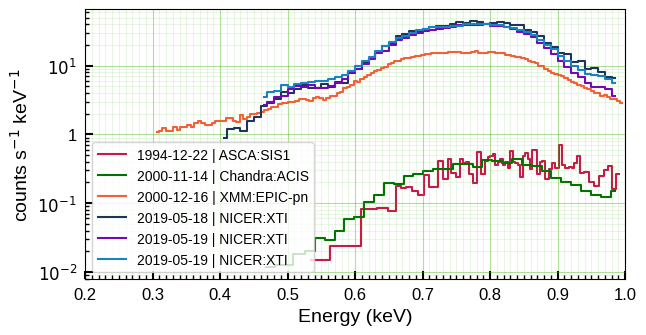
\includegraphics[width=\textwidth]{figures/ldata/mr-vel-counts_all-obs.png}
            \caption{Comparison of flux from all observations from their count rates plotted to scale}
            \label{fig:all-counts:unnorm}
        \end{subfigure}
        \hfill
        \begin{subfigure}[b]{0.45\textwidth}
            \centering
            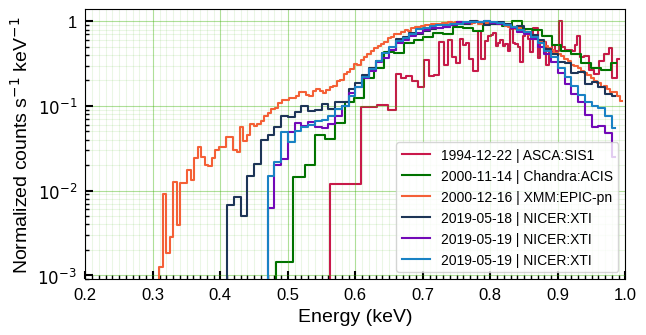
\includegraphics[width=\textwidth]{figures/ldata/mr-vel-normcounts_all-obs.png}
            \caption{Normalized count rates from all observations show varying responses to supersoft X-rays}
            \label{fig:all-counts:norm}
        \end{subfigure}
        \caption{Count rates from observational dataset}
        \label{fig:all-counts}
    \end{figure*}
    
    Concurrently, in figure \ref{fig:all-counts:norm}, the count rates are normalized to the range of 0 to 1 using \textit{min-max normalization}. This visualization accentuates the relative sensitivity of more recent observations to supersoft X-ray photons emitted by \source. The sub-plot shows that in recent observations the supersoft X-ray features are discernibly enhanced. This might be suggestive of improved observational capabilities or heightened sensitivity to the emitted X-ray flux.
    
    Together, these visualizations offer a nuanced understanding of the flux variability and observational sensitivity trends exhibited by \source\ across different observation epochs, contributing to the broader understanding of its X-ray emission characteristics.
    
    \subsection{NLTE continuum model}
    In table \ref{tab:res-fitting}, we present the luminosity, effective temperature and column density for \source\ which are derived after performing the fitting to the NLTE continuum model described in \S \ref{sec:reduction-analysis} We also present the model fit statistics, namely the reduced $\chi^2$ values for each fit. It can be noticed that the same continuum model has been able to provide a good fit to all of the observations in our chosen dataset.
    \begin{table*}[!htb]
    	\centering
    	\caption{Parameters of \source\ derived from continuum NLTE model from multi-observatory observations.}
    	\label{tab:res-fitting}
    	\begin{tabular}{ccccccc}
			\hline
			{\textbf{Observatory}} & {\textbf{Obs. ID}} & {$\boldsymbol{L_*}$ \textbf{(erg s$\boldsymbol{^{-1}}$)}} & {\textbf{$\boldsymbol{T_\text{eff}}$ (kK)}} & {\textbf{$\boldsymbol{n_H}$ ($\boldsymbol{\times 10^{22}}$ cm$\boldsymbol{^{-2}}$)}} & {$\boldsymbol{\chi^2}$/\textbf{d.o.f}} & {$\boldsymbol{\chi^2_\text{reduced}}$} \\
			\hline
			{ASCA} & {43036000} & {$2.07_{0.46}^{71.02}\times 10^{41}$} & {$100.2_{56.2}^{147.4}$} & {$0.13_{0.00}^{1.36}$} & {75.4/62} & {1.22} \\ %updated
			{Chandra} & {644} & {$4.38_{2.02}^{24.34}\times 10^{41}$} & {$96.3_{81.6}^{120.5}$} & {$1.25_{1.17}^{1.37}$} & {30.5/28} & {1.09} \\ %updated
			{XMM-Newton} & {0111150101} & {$2.19_{1.96}^{3.74}\times 10^{42}$} & {$91.7_{86.9}^{100.2}$} & {$1.17_{1.09}^{1.27}$} & {183.4/131} & {1.40} \\ %updated
			{NICER} & {2611020101} & {$8.40_{6.77}^{19.16}\times 10^{41}$} & {$100.8_{90.0}^{110.1}$} & {$1.22_{1.11}^{1.28}$} & {65.4/52} & {1.26} \\ %updated
			{NICER} & {2611020102} & {$1.68_{1.41}^{3.37}\times 10^{41}$} & {$99.8_{92.1}^{100.3}$} & {$0.51_{0.49}^{0.57}$} & {82.9/50} & {1.66} \\
			{NICER} & {2611020103} & {$4.41_{3.42}^{6.81}\times 10^{40}$} & {$107.8_{102.5}^{110.2}$} & {$0.28_{0.27}^{0.33}$} & {104.8/50} & {2.10} \\
			\hline
		\end{tabular}
	\end{table*}
    
    \subsection{Unfolded spectra}
    In figure \ref{fig:all-uf}, the unfolded spectrum, which is obtained after fitting the data to the best-fit model, is displayed. Observations in panels \ref{fig:all-uf:12-24} and \ref{fig:all-uf:24-36} reveal features which are indicative of the presence of elemental absorption edges.
    
    \begin{figure*}[!bht]
        \centering
        \begin{subfigure}[b]{0.45\textwidth}
            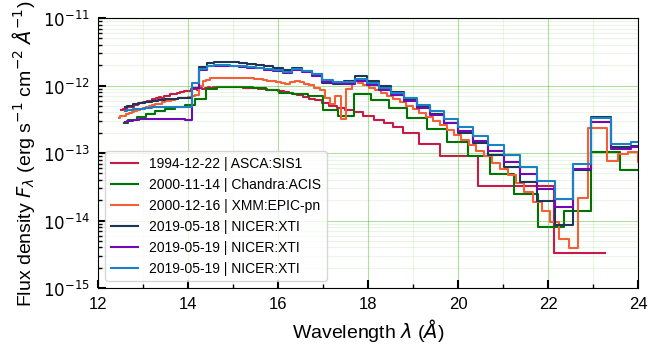
\includegraphics[width=\textwidth]{figures/eufspec/mr-vel-uf_all-obs_12-24.png}
            \caption{Unfolded spectra after model fitting in the range 12 \AA - 24 \AA}
            \label{fig:all-uf:12-24}
        \end{subfigure}
        \hfill
        \begin{subfigure}[b]{0.45\textwidth}
            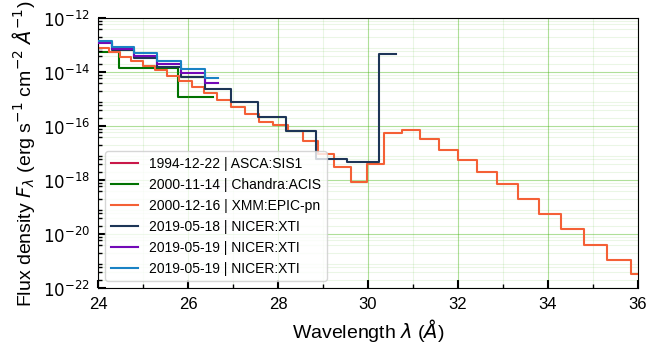
\includegraphics[width=\textwidth]{figures/eufspec/mr-vel-uf_all-obs_24-36.png}
            \caption{Unfolded spectra after model fitting in the range 24 \AA - 36 \AA}
            \label{fig:all-uf:24-36}
        \end{subfigure}
        \caption{Unfolded spectra after model fitting}
        \label{fig:all-uf}
    \end{figure*}
    
    \subsection{Luminosity versus effective temperature}
    \begin{figure}[!thb]
    	\centering
    	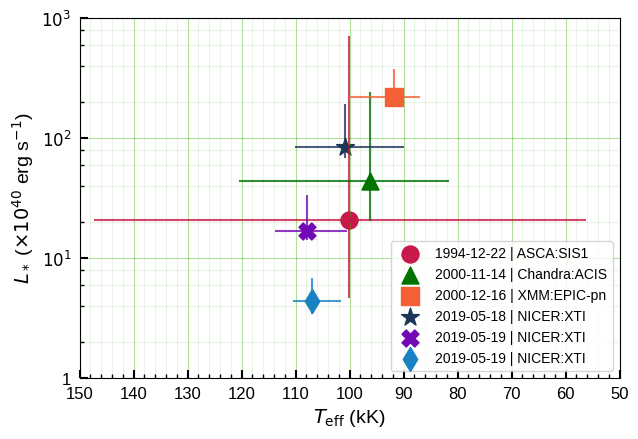
\includegraphics[width=0.5\textwidth]{figures/L-Teff_all-obs.png}
    	\caption{Uncertainties in $L_*$ and $T_\text{eff}$ calculations from multi-observatory observations of \source}
    	\label{fig:L-Teff}
    \end{figure}
    In figure \ref{fig:L-Teff}, we present a visualization of the calculated values of the luminosity $L_*$ and effective temperature $T_\text{eff}$ for \source\ using the best-fit model. One may note that the horizontal axis, containing the $T_\text{eff}$ data is plotted as increasing from right to left, \textit{\`{a} la} Hertzsprung-Russell diagram. This enables one to compare the overlap of the regions of uncertainty of these parameters as calculated using the data from multiple observatories.

    \subsection{Presence of elemental absorption edges}
    Four elemental absorption edges were detected upon the inspection of the unfolded spectra obtained from the best fitting model on all the observations. These absorption edges, belonging to N, O, Ne and Fe, are overlaid on the unfolded spectra and displayed in figure \ref{fig:all-uf:abs-edges}.
    \begin{figure*}[!htb]
        \centering
        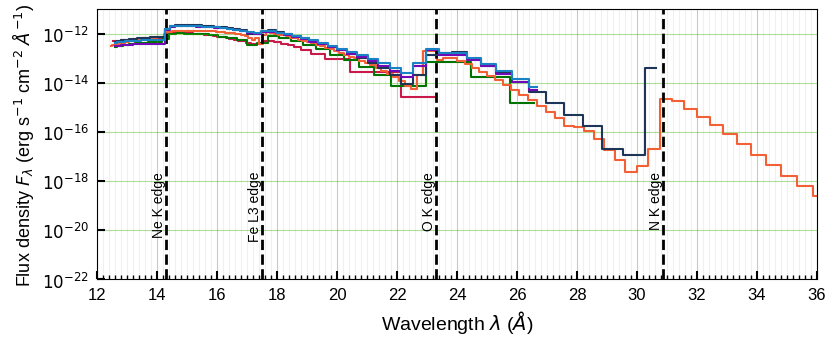
\includegraphics[width=0.8\textwidth]{figures/eufspec/mr-vel-uf-ang_abs-edge.png}
        \caption{Unfolded spectra with overlaid elemental absorption edges}
        \label{fig:all-uf:abs-edges}
    \end{figure*}
    
    \begin{table*}[!htb]
    	\centering
    	\caption{Absorption depth $D$ of \source\ derived from identified absorption edges of Ne, Fe, O and N.}
    	\label{tab:abs-depth}
		\begin{tabular}{cccccc}
			\hline
			\multirow{3}{*}{\textbf{Observatory}} & \multirow{3}{*}{\textbf{Obs. ID}} & \multicolumn{4}{c}{\textbf{Absorption Depth $\boldsymbol{D}$}} \\ \cline{3-6} & & \textbf{Ne $\boldsymbol{K}$ edge} & \textbf{Fe $\boldsymbol{L_3}$ edge} & \textbf{O $\boldsymbol{K}$ edge} & \textbf{N $\boldsymbol{K}$ edge} \\ \cline{3-6} & & \textbf{14.302 \AA} & \textbf{17.509 \AA} & \textbf{23.305 \AA} & \textbf{30.873 \AA} \\
			\hline
			{ASCA} & {43036000} & {0.503} & {0.661} & {0.941} & {1.787} \\ %updated
			{Chandra} & {644} & {0.497} & {0.673} & {1.823} & {5.171} \\ %updated
			{XMM-Newton} & {0111150101} & {0.211} & {0.033} & {0.132} & {5.215} \\ %updated
			{NICER} & {2611020101} & {0.819} & {0.000} & {1.630} & {0.185} \\ %updated
			{NICER} & {2611020102} & {1.524} & {0.208} & {0.476} & {1.755} \\
			{NICER} & {2611020103} & {1.244} & {0.304} & {0.485} & {5.003} \\
			\hline
		\end{tabular}
	\end{table*}

    Because the best-fitted spectrum obtained from the EPIC-pn instrument of XMM-Newton spans the widest range of wavelengths, known absorption edges \cite{bearden1967reevaluation,juett2006high} were identified in the vicinity of the absorption edges in figure \ref{fig:all-uf:abs-edges}. These are reported in table \ref{tab:abs-depth}. Then they were overlaid on the unfolded spectrum obtained from the EPIC-pn observation. The four absorption edges that could be identified are the $K$ edges of N, O and Ne and the $L_3$ edge of Fe at 30.873 \AA, 23.305 \AA, 14.302 \AA\ and 17.509 \AA\ respectively, as displayed in the sub-plots of figure \ref{fig:pn-uf:abs-edges}. Three among these four edges, namely the $K$ edges of O and Ne and the $L_3$ edge of Fe, were reported to be present in the spectrum of \source\ using the CLOUDY photoionization code by Prodhani and Baruah (2018) \cite{prodhani2018galactic}.

    \begin{figure*}[!bht]
        \centering
        \begin{subfigure}[b]{0.45\textwidth}
            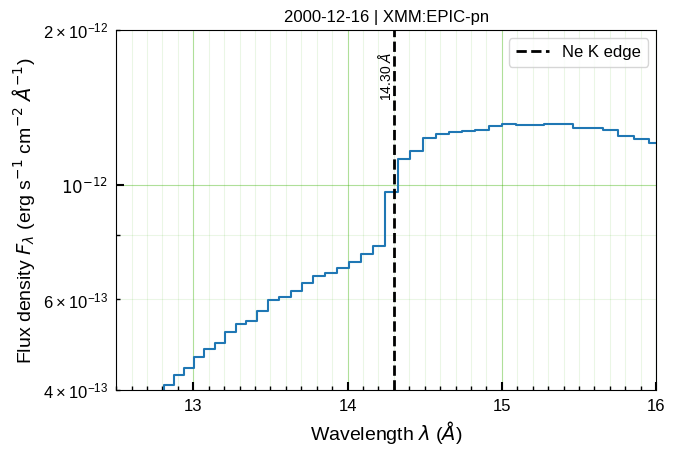
\includegraphics[width=\textwidth]{figures/eufspec/mr-vel-XMM-EPIC-pn-uf-Ne-edges.png}
            \caption{Ne K absorption edge at 14.302 \AA}
            \label{fig:pn-uf:Ne-edges}
        \end{subfigure}
        \hfill
        \begin{subfigure}[b]{0.45\textwidth}
            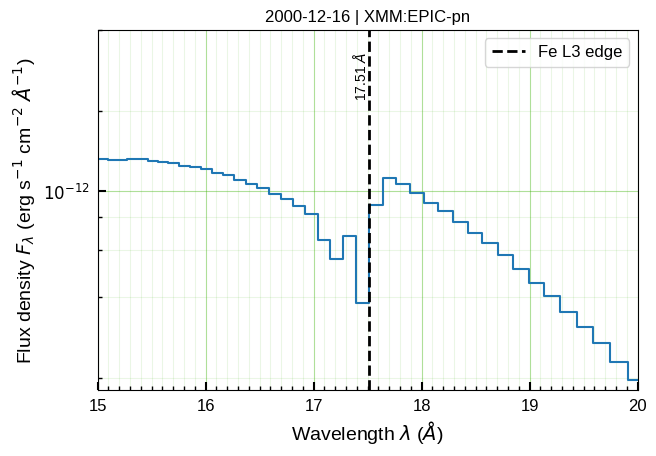
\includegraphics[width=\textwidth]{figures/eufspec/mr-vel-XMM-EPIC-pn-uf-Fe-edges.png}
            \caption{Fe L$_3$ absorption edge at 17.509 \AA}
            \label{fig:pn-uf:Fe-edges}
        \end{subfigure}
        \begin{subfigure}[b]{0.45\textwidth}
            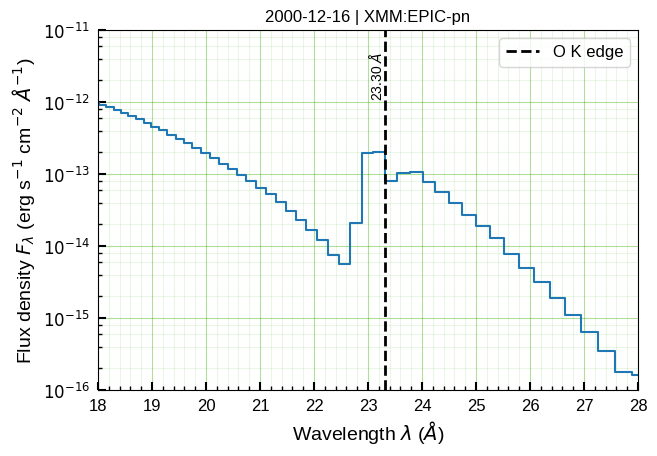
\includegraphics[width=\textwidth]{figures/eufspec/mr-vel-XMM-EPIC-pn-uf-O-edges.png}
            \caption{O K absorption edge at 23.305 \AA}
            \label{fig:pn-uf:O-edges}
        \end{subfigure}
        \hfill
        \begin{subfigure}[b]{0.45\textwidth}
            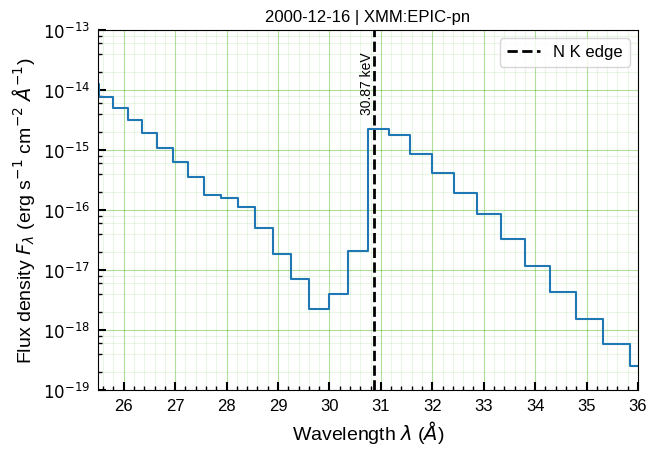
\includegraphics[width=\textwidth]{figures/eufspec/mr-vel-XMM-EPIC-pn-uf-N-edges.png}
            \caption{N K absorption edge at 30.873 \AA}
            \label{fig:pn-uf:N-edges}
        \end{subfigure}
        \caption{Absorption edges for N, O, Ne and Fe overlaid on the unfolded spectrum for EPIC-pn observation}
        \label{fig:pn-uf:abs-edges}
    \end{figure*}
